% !TeX root = ../main.tex

\section{Introduzione}
In questo capitolo vengono mostrati i risultati ottenuti dalla realizzazione della applicazione multipiattaforma MaggioliEbook adottando il processo di sviluppo descritto nel capitolo \ref{ch:cicd}.

Vengono inizialmente considerati i requisiti definiti nel capitolo \ref{ch:casodistudio} e paragonati con quanto realizzato. Successivamente sono indicate alcune statistiche e metriche, raccolte principalmente tramite la piattaforma GitLab adottata, al fine di creare un primo modello di confronto per i lavori futuri che saranno svolti in azienda sulle tematiche principali di questo caso di studio industriale.

\section{Riuso}
I template che definiscono gli stage e i relativi job del processo di sviluppo progettato sono stati versionati e organizzati in un apposito repository, come descritto in modo dettagliato nel capitolo \ref{ch:cicd}.

Questa soluzione non solo permette il riuso dell'intera pipeline o di solamente una sua parte, ma abilita anche un processo di lavoro collaborativo fra tutti i possibili utilizzatori per la modifica del processo. Ogni sviluppatore all'interno della azienda è infatti in grado di accedere al repository dei template, visionare i file YAML che definiscono la pipeline e aprire merge request per richiedere la modifica o l'aggiunta di funzionalità necessarie al processo di sviluppo automatizzato. A tal proposito è stato scelto un team di sviluppo all'interno dell'azienda che si occupa di applicazioni mobile per svolgere un primo esperimento di integrazione nel proprio processo di sviluppo, già consolidato su tecnologie puramente native e senza alcun sistema di automazione.

\section{Stabilizzazione e rilascio}
La fase di stabilizzazione e rilascio di entrambe le versioni di applicazione sviluppate tramite Kotlin Multiplatform Mobile sono state realizzate rispettando tutti i vincoli definiti nel capitolo \ref{ch:casodistudio}. Durante il processo di sviluppo del caso di studio è stato infatti possibile rilasciare automaticamente applicazioni, sia Android che iOS, sfruttando la pipeline realizzata. In entrambi i casi sono stati definiti gruppi di tester composti sia dalle figure aziendali esperte di dominio che dai Professori relatori di questa tesi:

\begin{figure}[H]
    \centering
    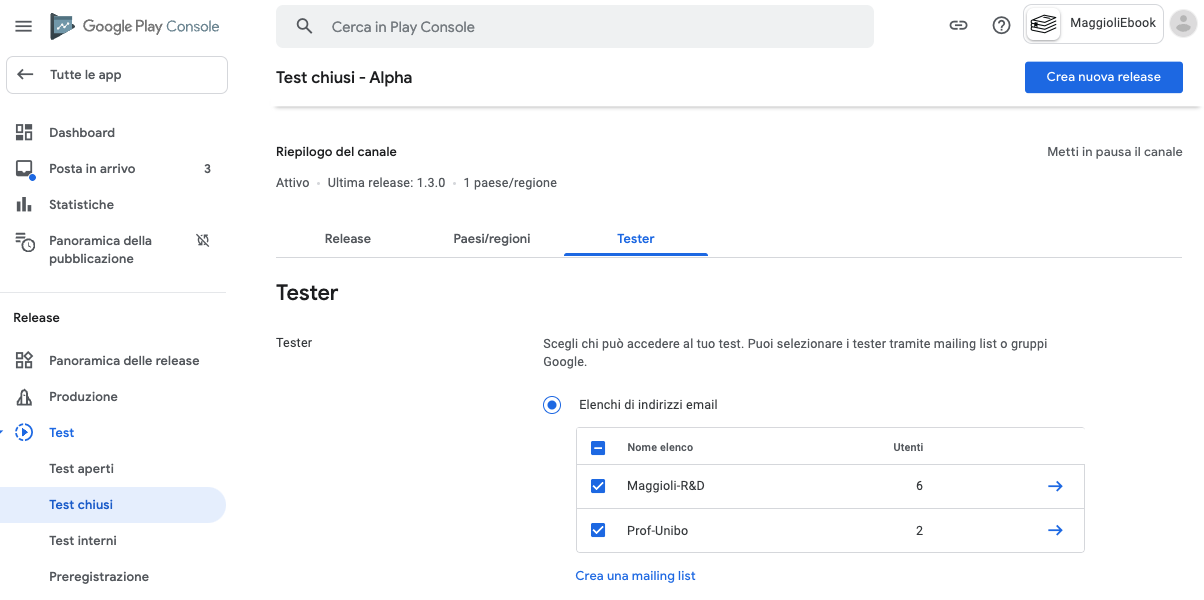
\includegraphics[width=1\textwidth]{img/google-play-console-maggioliebook.png}
    \caption{Schermata Google Play Console per la fase di stabilizzazione della applicazione Android}
    \label{google-play-console-maggioliebook}
\end{figure}

\begin{figure}[H]
    \centering
    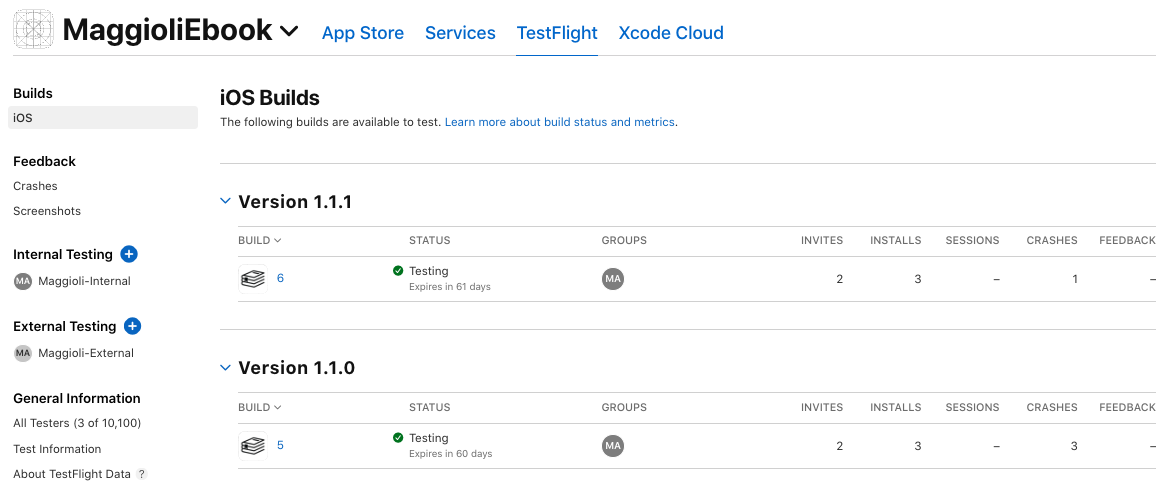
\includegraphics[width=1\textwidth]{img/app-store-connect-maggioliebook.png}
    \caption{Schermata App Store Connect per la fase di stabilizzazione della applicazione iOS}
    \label{app-store-connect-maggioliebook}
\end{figure}

Tutti i tester appartenenti ai gruppi configurati come nelle schermate precedenti sono poi stati in grado di installare con successo l'applicazione sul proprio dispositivo:

\begin{figure}[H]
    \centering
    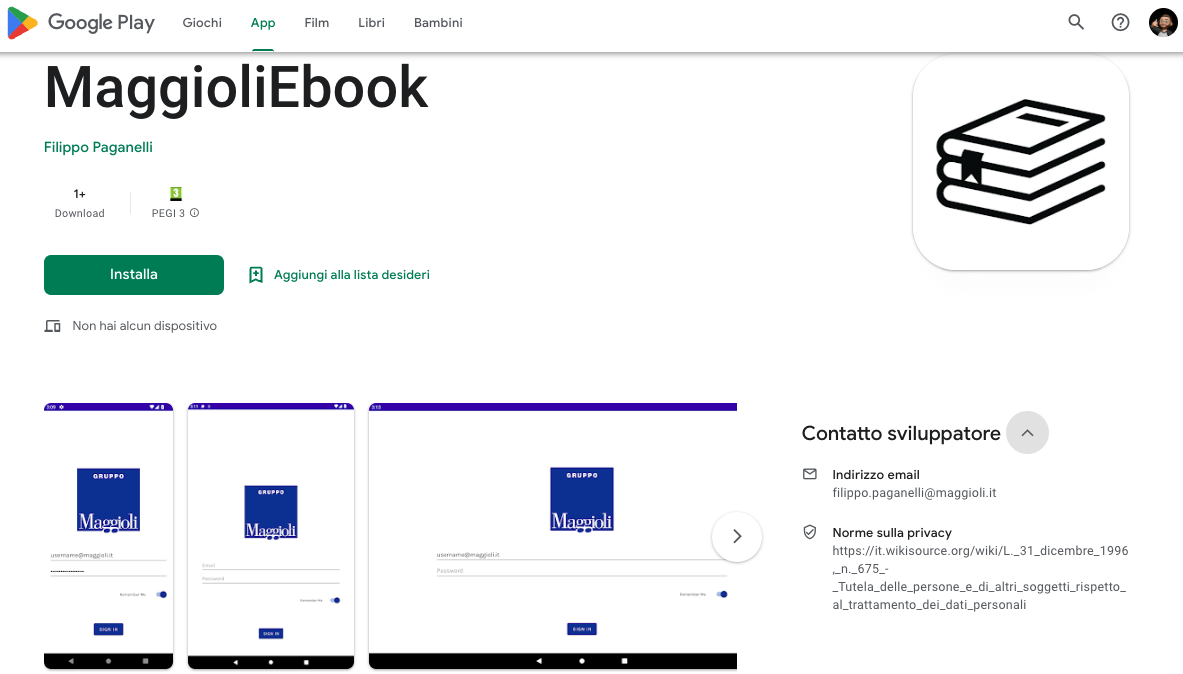
\includegraphics[width=1\textwidth]{img/google-play-store-maggioliebook.png}
    \caption{Schermata Google Play Store per la fase di stabilizzazione della applicazione Android}
    \label{google-play-store-maggioliebook}
\end{figure}

\begin{figure}[H]
    \centering
    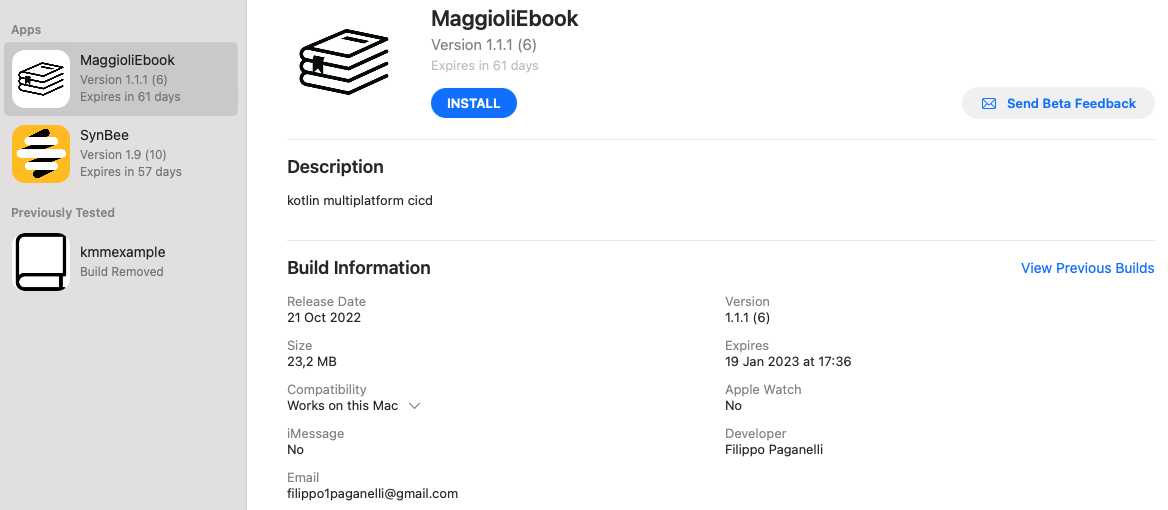
\includegraphics[width=1\textwidth]{img/testflight-maggioliebook.png}
    \caption{Schermata Testflight per la fase di stabilizzazione della applicazione iOS}
    \label{testflight-maggioliebook}
\end{figure}

Un ciclo di stabilizzazione \textit{alpha}-\textit{beta} risulta nell'esecuzione di due pipeline attivate rispettivamente con (\textit{i}) la modifica sul branch \textit{dev} del codice della applicazione e (\textit{ii}) il merge del branch \textit{dev} sul branch \textit{test}. Le seguenti schermate, catturate dalla piattaforma GitLab utilizzata come sistema di versionamento e automazione, mostrano l'esecuzione di un esempio di queste due pipeline nel caso della sola applicazione Android:

\begin{figure}[H]
\centering
    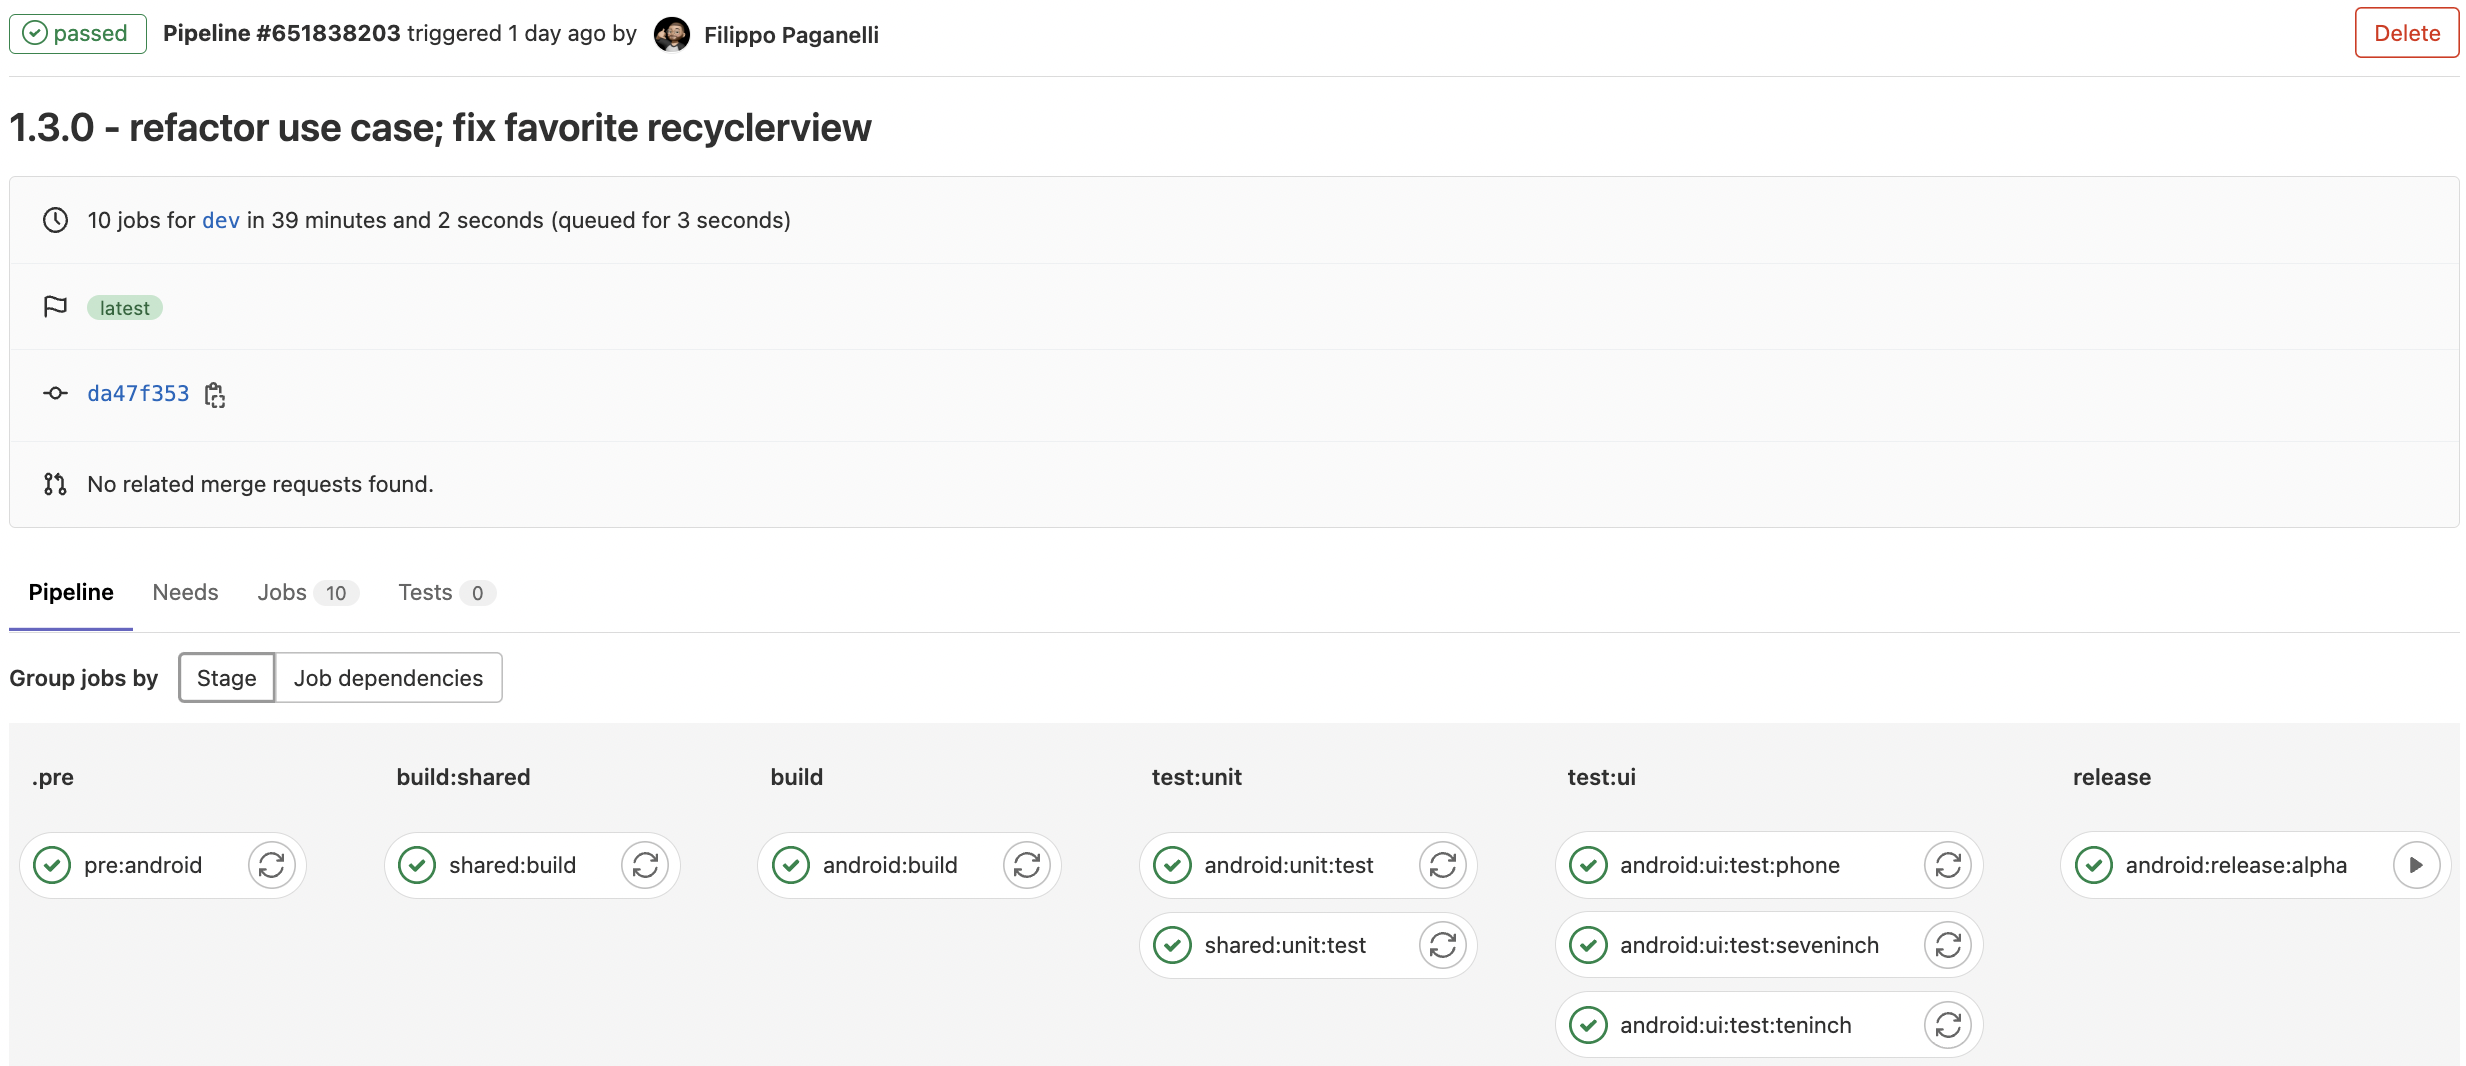
\includegraphics[width=1\textwidth]{img/gitlab-pipeline-android-alpha.png}
    \caption{Schermata GitLab di esecuzione della pipeline completa per il rilascio della applicazione Android in versione \textit{alpha}}
    \label{gitlab-pipeline-android-alpha}
\end{figure}

\begin{figure}[H]
\centering
    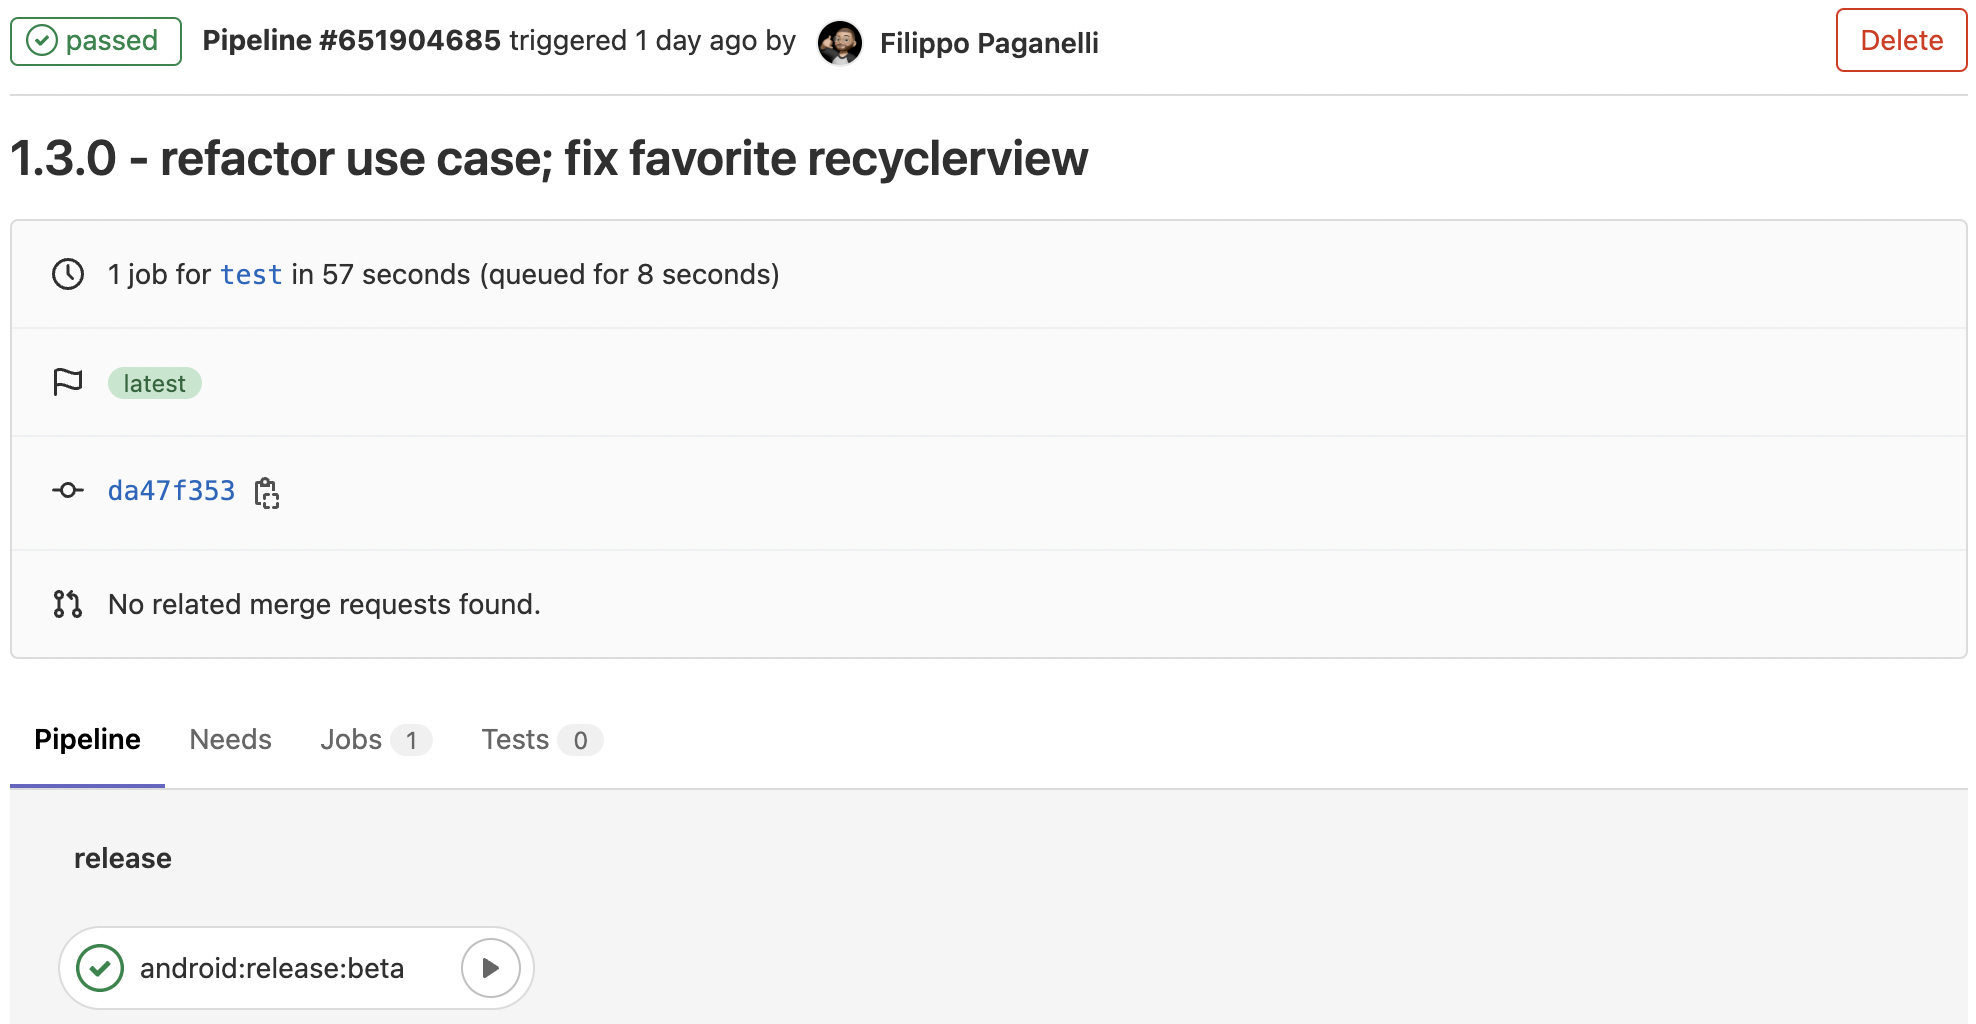
\includegraphics[width=1\textwidth]{img/gitlab-pipeline-android-beta.png}
    \caption{Schermata GitLab di esecuzione della pipeline completa per la promozione da versione \textit{alpha} a versione \textit{beta} della applicazione Android}
    \label{gitlab-pipeline-android-beta}
\end{figure}

\section{Analisi del codice}
La fase di analisi del codice è stata realizzata con successo seguendo i vincoli aziendali e le pratiche di Continuous Inspection come descritto rispettivamente nei capitoli \ref{ch:casodistudio} e \ref{ch:cicd}. La seguente schermata catturata dalla piattaforma GitLab rappresenta l'esecuzione di una pipeline schedulata per l'analisi del codice terminata con successo:

\begin{figure}[H]
\centering
    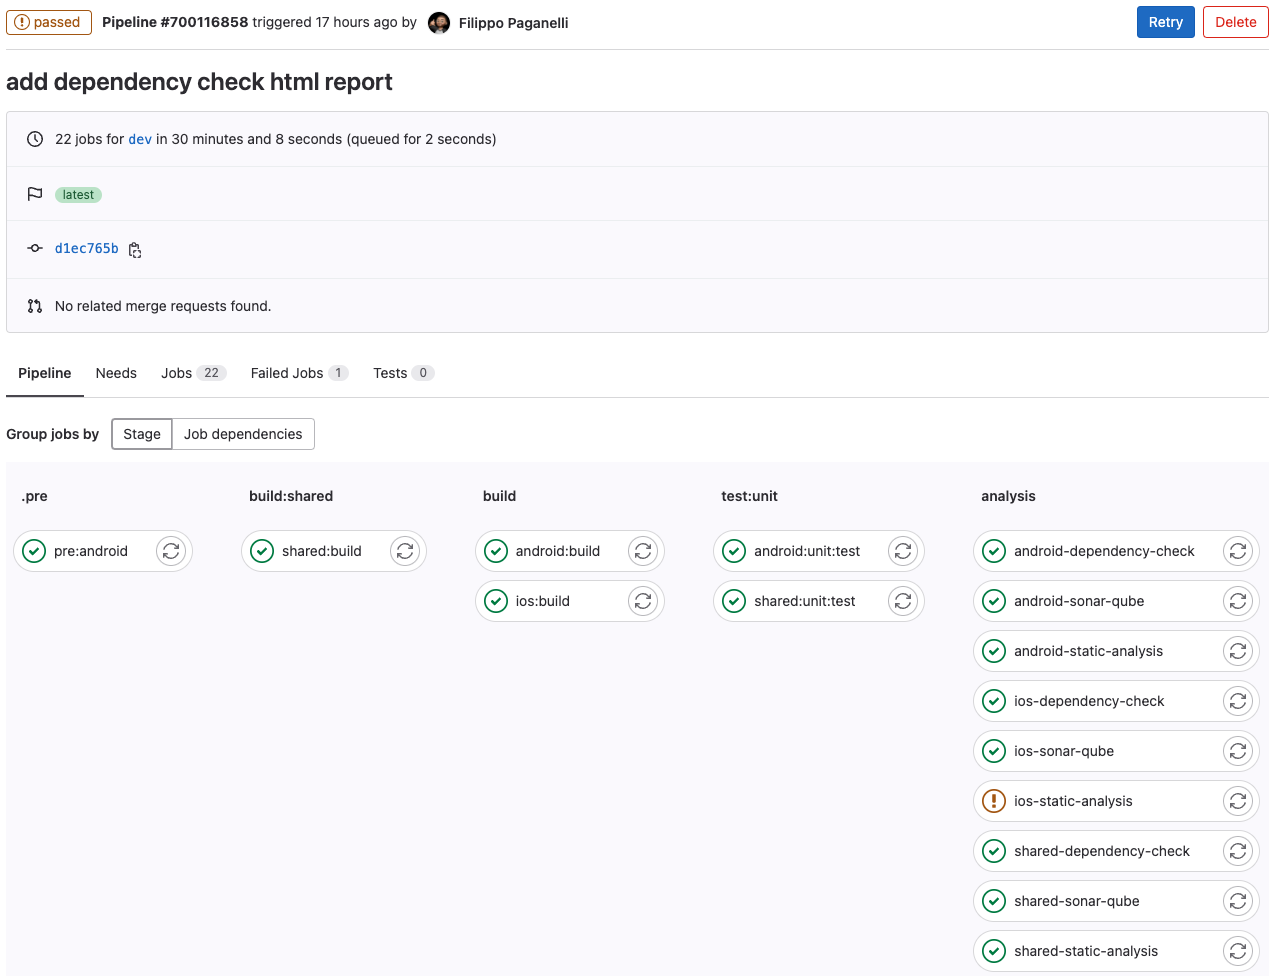
\includegraphics[width=1\textwidth]{img/gitlab-pipeline-analysis.png}
    \caption{Schermata GitLab di esecuzione della pipeline completa per l'analisi del codice dei tre moduli sviluppati}
    \label{gitlab-pipeline-analysis}
\end{figure}

Nonostante il sistema di automazione implementato per questa fase di analisi funzioni correttamente come atteso, non è possibile dire lo stesso per i risultati ottenuti dalle scansioni dei vari tools utilizzati, come Dependency-Check, Detekt e SwiftLint, e soprattutto per la loro integrazione con il servizio aziendale SonarQube:

\begin{figure}[H]
\centering
    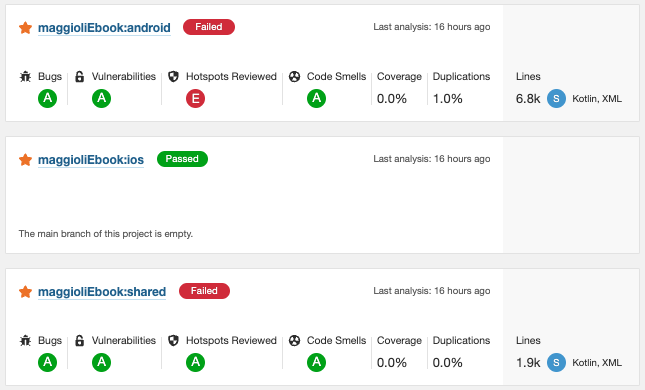
\includegraphics[width=0.9\textwidth]{img/sonarqube-kmm.png}
    \caption{Schermata SonarQube aziendale contenente i tre moduli del caso di studio analizzati}
    \label{sonarqube-kmm}
\end{figure}

Per esempio, nella seguente schermata rappresentante la panoramica del progetto iOS è indicata la presenza di 837 risultati classificati come \textit{code smells} dei quali 815 con severity \textit{minor} e 22 con severity \textit{major} ma nella schermata precedente, ovvero la Homepage del servizio SonarQube aziendale, non è indicato alcun risultato.

\begin{figure}[H]
\centering
    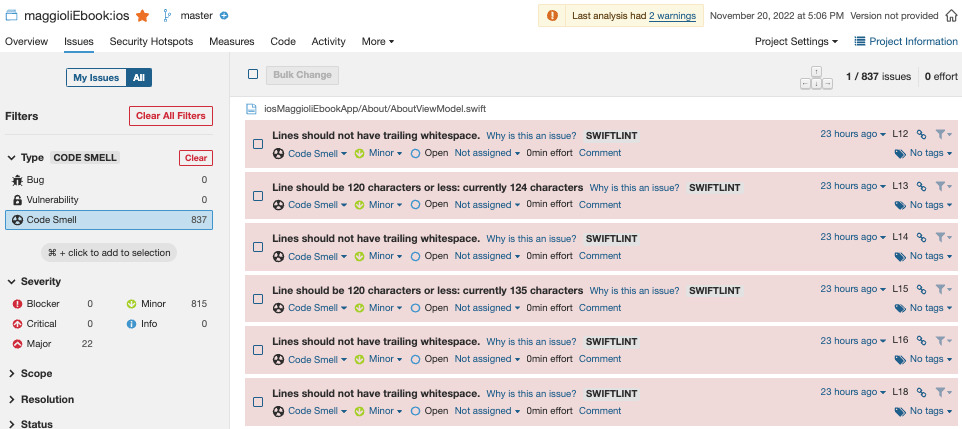
\includegraphics[width=1\textwidth]{img/sonarqube-ios.png}
    \caption{Schermata SonarQube aziendale in cui è mostrata la panoramica del progetto iOS e i risultati ottenuti dalle scansioni tramite il tool SwiftLint}
    \label{sonarqube-ios}
\end{figure}

\section{Statistiche}
Considerando il contesto in cui è stato realizzato il caso di studio industriale è molto complesso estrarre metriche e valori confrontabili: gli esistenti team di sviluppo in azienda che si occupano di applicazioni mobile al momento non adottano nessuna tecnologia moderna per lo sviluppo multi-platform o cross-platform e nessun sistema di automazione per il processo.

L'adozione della cultura DevOps e l'applicazione delle pratiche abilitanti, come descritto nel capitolo \ref{ch:devops}, in ambito mobile utilizzando moderne tecniche di sviluppo multipiattaforma, come indicato nel capitolo \ref{ch:app-multiplatform}, consiste in un progetto di forte innovazione realizzato nel contesto aziendale di Ricerca e Sviluppo. Tipicamente sia le risorse assegnate a questi progetti che la complessità dei domini modellati non sono paragonabili ai prodotti commercializzati dalle altre business unit aziendali ma sono tarati per lo sviluppo di progetti dimostrativi, conosciuti anche come \textit{Proof of Concept}.

Le seguenti metriche e statistiche indicate, raccolte tramite l'ausilio della piattaforma GitLab utilizzata, forniscono dunque un analisi del caso di studio definendo un punto di partenza per il confronto dei lavori futuri svolti nelle stesse aree tematiche e indicate nella sezione successiva.

\subsection*{Percentuale linguaggi utilizzati}
La seguente metrica, fornita dal servizio GitLab \textit{Repository Analytics}\footnote{\href{https://docs.gitlab.com/ee/user/analytics/repository\_analytics.html}{https://docs.gitlab.com/ee/user/analytics/repository\_analytics.html}}, definisce la composizione del repository contenente il sorgente della applicazione KMM MaggioliEbook (capitolo \ref{ch:maggioliebook}) in termini di percentuale di linguaggi di programmazione utilizzati: 57,38\% Kotlin, 42,09\% Swift e 0,54\% Ruby.

\begin{figure}[H]
\centering
    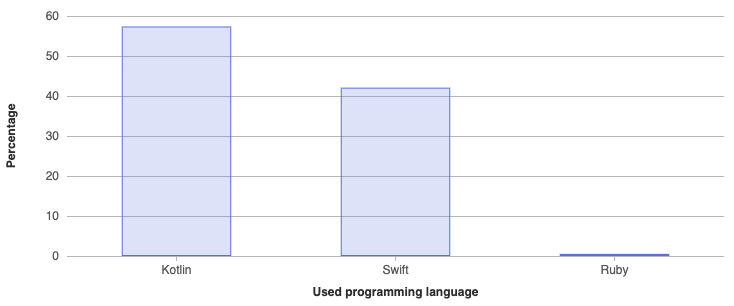
\includegraphics[width=1\textwidth]{img/repo-code-lang-percent.png}
    \caption{Composizione del repository della applicazione KMM MaggioliEbook in termini di percentuale di linguaggi di programmazione utilizzati}
    \label{repo-code-lang-percent}
\end{figure}

\subsection*{Commit effettuate e distribuzione temporale}
Anche le seguenti metriche sono fornite dallo stesso servizio GitLab \textit{Repository Analytics} e definiscono la distribuzione temporale delle commit effettuate sul repository della applicazione KMM MaggioliEbook.

E' importante considerare che i valori indicati nei seguenti grafici si riferiscono ad un totale di 185 commit realizzate da un solo autore nel periodo compreso tra il 17 Luglio 2022 (data di creazione del repository) e il 20 Novembre 2022.

\begin{figure}[H]
\centering
    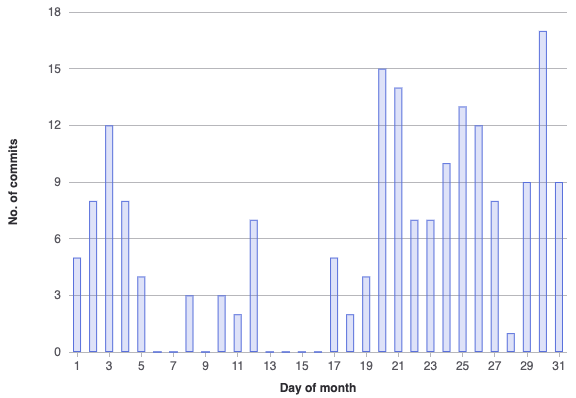
\includegraphics[width=0.7\textwidth]{img/commit-per-day-of-month.png}
    \caption{Distribuzione delle commit effettuate per giorno del mese}
    \label{commit-per-day-of-month}
\end{figure}

\begin{figure}[H]
\centering
    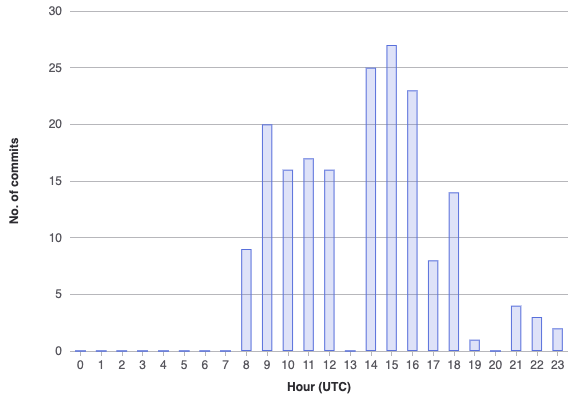
\includegraphics[width=0.7\textwidth]{img/commit-per-day-hour.png}
    \caption{Distribuzione delle commit effettuate per ora del giorno}
    \label{commit-per-day-hour}
\end{figure}

\subsection*{Tasso di successo delle pipeline}
La seguente metrica e quelle successive sono estratte da GitLab tramite un altro servizio, chiamato \textit{CI/CD Analytics}\footnote{\href{https://docs.gitlab.com/ee/user/analytics/ci\_cd\_analytics.html}{https://docs.gitlab.com/ee/user/analytics/ci\_cd\_analytics.html}}. Il tasso di successo delle pipeline eseguite per l'applicazione KMM MaggiolieBook è del 45,71\% ed è dato dal numero di pipeline terminate con successo (16) sul totale delle pipeline eseguite (35). Dal grafico è possibile notare che dopo un primo periodo di integrazione e adattamento della pipeline progettata tramite template, come descritto nel capitolo \ref{ch:cicd}, il tasso di successo è aumentato da circa il 16,67\% a Settembre 2022 a circa 45,71\% a Novembre 2022.

\begin{figure}[H]
\centering
    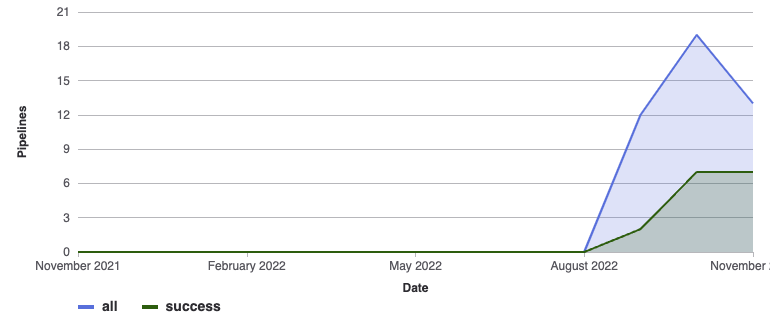
\includegraphics[width=0.9\textwidth]{img/gitlab-pipeline-chart.png}
    \caption{Tasso di successo delle pipeline (Luglio 2022 - Novembre 2022)}
    \label{gitlab-pipeline-chart}
\end{figure}

\subsection*{Durata delle pipeline per le ultime 30 commit effettuate}
Un altro grafico interessante fornito dal servizio GitLab \textit{CI/CD Analytics} è la durata delle pipeline eseguite per le ultime 30 commit per le quali era associata una regola di attivazione.

\begin{figure}[H]
\centering
    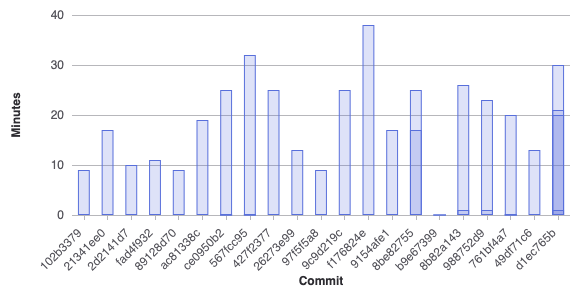
\includegraphics[width=0.75\textwidth]{img/gitlab-cicd-stats.png}
    \caption{Durata delle pipeline per le ultime 30 commit effettuate sul repository della applicazione KMM MaggioliEbook}
    \label{gitlab-cicd-stats}
\end{figure}

\subsection*{Durata media delle pipeline per fase di sviluppo e piattaforma coinvolta}
Considerando che le pipeline possono coinvolgere una o entrambe le versioni della applicazione sviluppata in base alla modifica effettuata al codice, una metrica utile a future valutazioni e confronti è data dal tempo medio di esecuzione delle pipeline in base alla piattaforma coinvolta, ovvero Android e/o iOS, e alla fase del processo: (\textit{i}) rilascio versione \textit{alpha}, (\textit{ii}) rilascio versione beta e (\textit{iii}) analisi statica del codice.

I seguenti valori sono stati calcolati utilizzando le tempistiche di esecuzione delle pipeline rilevate dalla piattaforma GitLab utilizzata.

\begin{table}[H]
\centering
    \begin{tabular}{|c|c|c|c|}
         \hline
         \textbf{Piattaforma} & \textbf{Rilascio Alpha} & \textbf{Rilascio Beta} & \textbf{Analisi}\\
         \hline
         Android & $\sim$ \textit{20 min} & $\sim$ \textit{1 min} & $\sim$ \textit{15 min} \\
         \hline
         iOS & $\sim$ \textit{23 min} & $\sim$ \textit{30 sec} & $\sim$ \textit{15 min} \\
         \hline
         Android e iOS & $\sim$ \textit{28 min} & $\sim$ \textit{1 min} & $\sim$ \textit{20 min} \\
         \hline
    \end{tabular}
    \caption{Durata media delle pipeline per fase di sviluppo e piattaforma coinvolta}
\end{table}

Per valutare queste metriche correttamente è necessario considerare gli stage e i job che compongono le varie fasi, come descritto nel capitolo \ref{ch:cicd}. La fase \textit{Rilascio Alpha} è la più lunga ed è composta infatti da tutti gli stage e i job che comprendono le pratiche di Continuous Integration e Continuous Delivery. La fase \textit{Rilascio Beta} svolge invece il solo compito di promozione di una versione da \textit{alpha} a \textit{beta} e per questo è molto più breve rispetto la precedente. L'ultima fase per cui sono state definite le metriche è quella di analisi, la quale deve eseguire tutti i job di analisi statica del codice e delle dipendenze per ognuna delle piattaforme.

\section{Lavori futuri}
I risultati descritti nella sezione precedente sono decisamente positivi, soprattutto in termini di processo di sviluppo e di sistema di automazione realizzato. L'intero sistema attualmente è basato su una infrastruttura ridotta, dedicata alla sola riuscita del caso di studio. Dalla re-ingegnerizzazione di quest'ultima al fine di renderla abbastanza robusta e scalabile per supportare realmente gli altri team di sviluppo in azienda che si occupano di applicazioni mobile è normale attendersi grandi miglioramenti in termini di prestazioni. A tal proposito, come già anticipato nel capitolo \ref{ch:cicd}, è necessario valutare le possibili alternative al componente GitLab runner self-hosted adottato come ad esempio soluzioni complete, virtual machine macOS e runner forniti as-a-Service.

Altri aspetti importanti riguardanti il processo di sviluppo e il sistema di automazione trattati sicuramente nei lavori futuri sono il monitoraggio e la configurazione remota\footnote{\href{https://firebase.google.com/docs/remote-config}{https://firebase.google.com/docs/remote-config}}. Il monitoraggio, come descritto nel capitolo \ref{ch:sdlc}, è la fase del processo di sviluppo che segue alla fase di distribuzione delle applicazioni e permette di monitorare sia il comportamento del dispositivo che quello dell'utente applicando tecniche e pratiche che rispettano la cultura DevOps (capitolo \ref{ch:devops}). La configurazione remota è un meccanismo che permette di ottimizzare l'intero processo di sviluppo poiché permette di modificare aspetti della applicazione in modo dinamico senza dover rilasciare nuove versioni: un tipico esempio di utilizzo è la configurazione dell'url di connessione al database (\textit{JDBC}\footnote{Java DataBase Connectivity}), effettuata ogni volta che viene migrato il database evitando valori cablati nel codice della applicazione.

Nonostante i buoni risultati ottenuti a livello generale di lavoro svolto è stata evidenziata nella sezione precedente la carenza nei report restituiti dalle fasi di analisi statica e nella loro integrazione con il Vulnerability Management System aziendale. Questo rappresenta un requisito importante per l'azienda e che per essere soddisfatto necessita di ulteriori approfondimenti.

Per quando riguarda invece lo sviluppo della applicazione mobile multipiattaforma, i risultati raggiunti tramite il framework Kotlin Multiplatform Mobile sono stati soddisfacenti ma hanno dimostrato, soprattutto nel capitolo \ref{ch:maggioliebook}, che la condivisione di logica tra gli ecosistemi Android e iOS richiede ancora qualche miglioramento. Di fatto il framework KMM e tutti i componenti che utilizza, come il compilatore Kotlin/Native e i plugin Gradle, sono tutti in fasi \textit{pre-stable}.

Al fine di completare lo studio e la sperimentazione sulle moderne tecniche di sviluppo di applicazioni mobile e sulle pratiche DevOps ad esse applicabili è necessario sviluppare lo stesso caso di studio industriale tramite l'utilizzo dei framework cross-platform, come ad esempio quelli indicati nel capitolo \ref{ch:app-multiplatform} e la realizzazione di altri template per il riuso della pipeline nel caso di sviluppo con questi framework.
